%\documentclass[aspectratio=169]{beamer}
\documentclass{beamer}

\usetheme{mpcshpc}

\usepackage{lmodern}
\usepackage{listings}
\usepackage{hyperref}
\usepackage[scale=2]{ccicons}
\usepackage{minted}
\usepackage{multirow}
\usepackage{graphicx}
\usepackage{caption}
\usepackage{amsmath}
\usepackage{biblatex}
\usepackage{makecell}
\graphicspath{{./img/}}

\title{Async 4: Timing and Shared Memory in a Dot Product Implementation}
\subtitle{MPCS 51087: High-Performance Computing}
\date{Winter 2021}
\author{Ron Rahaman}
\institute{The University of Chicago, Dept of Computer Science}

\setwatermark{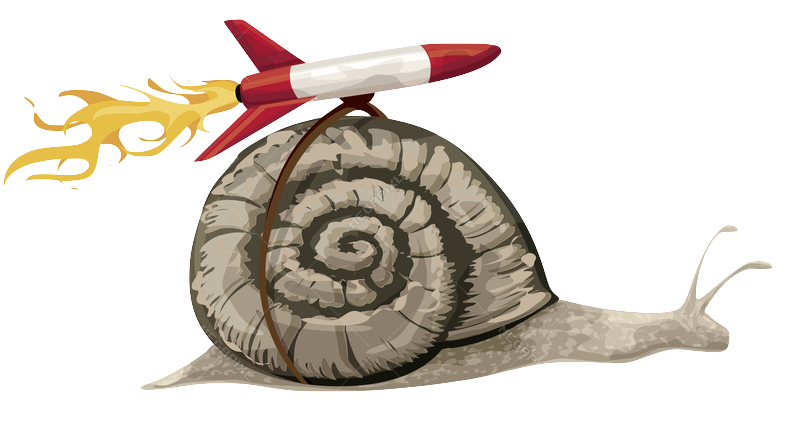
\includegraphics[height=7cm]{img/snail-rocket}}
\setminted{fontsize=\footnotesize}

\AtBeginSection[]
{
\begin{frame}
    \frametitle{Table of Contents}
    \tableofcontents[currentsection]
\end{frame}
}


\AtBeginSubsection[]
{
\begin{frame}
    \frametitle{Table of Contents}
    \tableofcontents[currentsubsection]
\end{frame}
}


\begin{document}

    \maketitle

    \begin{frame}
        \frametitle{Table of Contents}
        \tableofcontents[]
    \end{frame}

    \section{Timing GPU Code}

    \begin{frame}{Using host timers for GPU kernels?}
        \begin{itemize}
            \item You cannot reliably time GPU kernels using CPU timers (\texttt{clock\_gettime}, \texttt{std::chrono}, etc.) because because many CUDA commands are asynchronous.
            \item When the CPU calls an \textbf{asynchronous} GPU kernel or function, the CPU can continue to execute other tasks before the GPU is finished executing that funtion.
            \begin{itemize}
                \item Kernel launches are asynchronous.
            \end{itemize}
            \item When the CPU calls a \textbf{blocking} GPU function, the CPU must wait until until the GPU function is finished.
            \begin{itemize}
                \item Regular memcopies (\texttt{cudaMemcpy}) are blocking.
            \end{itemize}
        \end{itemize}
    \end{frame}

    \begin{frame}{Example: Which timings are reliable?}
        \begin{itemize}
            \item Is the time measured between \texttt{start} and \texttt{kernel\_end} reliable?
            \item What about the time measured between \texttt{start} and \texttt{memcpy\_end}?
        \end{itemize}
        \begin{block}{}
            \inputminted{cuda}{src/cpu-timer.cu}
        \end{block}
    \end{frame}

    \begin{frame}{GPU Timing with CUDA Events}
        \begin{itemize}
            \item During execution on the GPU, CUDA \textbf{events} can be used to reliably time CUDA \textbf{streams}.
            \item Events and streams have many complex usages, but basic usage for timing is very simple.
        \end{itemize}
    \end{frame}

    \begin{frame}{Basics of Streams and Events}
        \begin{columns}
            \begin{column}{0.6\textwidth}
                \begin{itemize}
                    \item A CUDA \textbf{stream} is an ordered queue of commands that execute on the GPU.
                    \begin{itemize}
                        \item Always at least one stream executing on the GPU (``default stream'', ``stream 0'', or ``NULL stream'')
                        \item Programmer can create additional streams for asynchronous commands.
                        \item Commands on the default stream implicitly block other streams.
                    \end{itemize}
                    \item A CUDA \textbf{event} is a timestamp recorded by the GPU on a specified stream.
                    \item By placing events on the default stream, we can reliably time the GPU.
                \end{itemize}
            \end{column}
            \begin{column}{0.4\textwidth}
                \begin{figure}
                    \centering
                    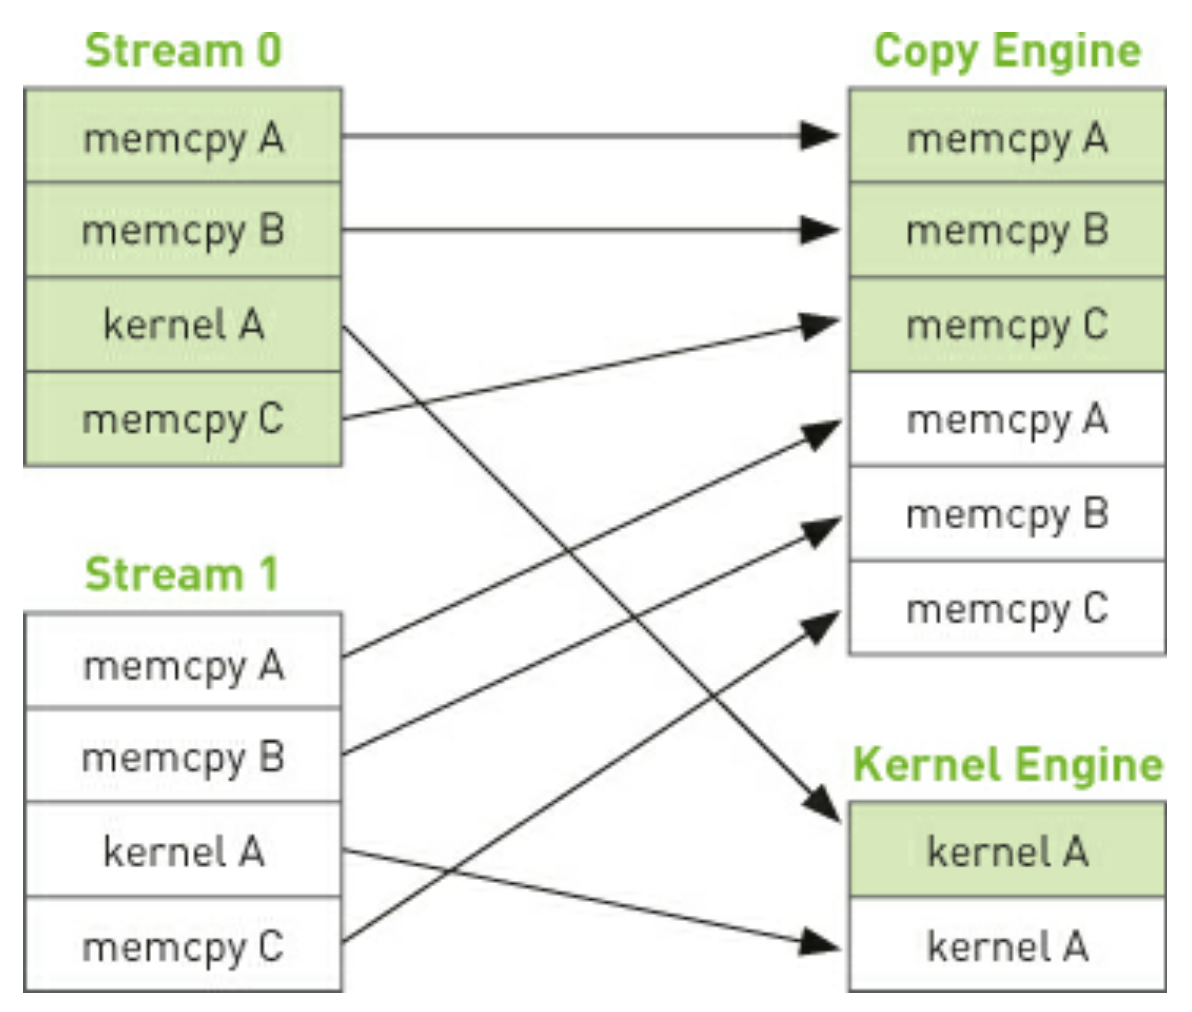
\includegraphics[width=\textwidth]{img/04/cu-by-ex-10-3.png}
                \end{figure}
            \end{column}
        \end{columns}
    \end{frame}

    \begin{frame}{Using Event-based Timers}
        \begin{columns}
            \begin{column}{0.4\textwidth}
            {\footnotesize
            \begin{itemize}
                \item \texttt{cudaEventCreate} initializes add \texttt{cudaEvent\_t} object
                \item \texttt{cudaEventRecord(tick, 0)}:  Queues-up the first event on stream 0
                \item \texttt{kernel}: Queues-up the kernel execution on stream 0
                \item \texttt{cudaEventRecord(tock, 0)}: Queues-up second event on stream 0
            \end{itemize}
            }
            \end{column}
            \begin{column}{0.6\textwidth}
                \begin{block}{}
                    \inputminted{cuda}{src/gpu-timer.cu}
                \end{block}
            \end{column}
        \end{columns}
    \end{frame}

    \begin{frame}{Using Event-based Timers, cont.}
        \begin{columns}
            \begin{column}{0.4\textwidth}
            {\footnotesize
            \begin{itemize}
                \item \texttt{cudaEventElapsedTime} returns the elapsed wall time between two events (in milliseconds)
                \item But first, we need to call \texttt{cudaEventSynchronize}!
                \item \texttt{cudaEventRecord} is an asynchronous command
                \item We need to make sure we call \texttt{cudaEventElapsedTime} after the event \texttt{tock} has actually finished.
            \end{itemize}
            }
            \end{column}
            \begin{column}{0.6\textwidth}
                \begin{block}{}
                    \inputminted{cuda}{src/gpu-timer.cu}
                \end{block}
            \end{column}
        \end{columns}
    \end{frame}

    \section{Intro to Shared Memory}

    \begin{frame}{Review: Abstraction/Hardware Mapping}
        \begin{columns}
            \column{0.5\textwidth}
            {\footnotesize
            \begin{itemize}
                \item \textbf{Thread (yellow)}
                \begin{itemize}
                    \item 1 thread assigned to 1 SP
                \end{itemize}
                \item \textbf{Warp (red)}
                \begin{itemize}
                    \item Contains multiple threads.  Number is hardware-specific.
                    \item $\ge 1$ warps assigned to 1 SM
                \end{itemize}
                \item \textbf{Block (blue)}
                \begin{itemize}
                    \item Contains multiple threads. Number is set by programmer at kenrel launch.
                    \item Contains multiple warps.  Number is implicitly determined by block dim and warp size.
                    \item $\ge 1$ blocks assigned to 1 SM
                \end{itemize}
            \end{itemize}
            }
            \column{0.5\textwidth}
            \begin{figure}
                \centering
                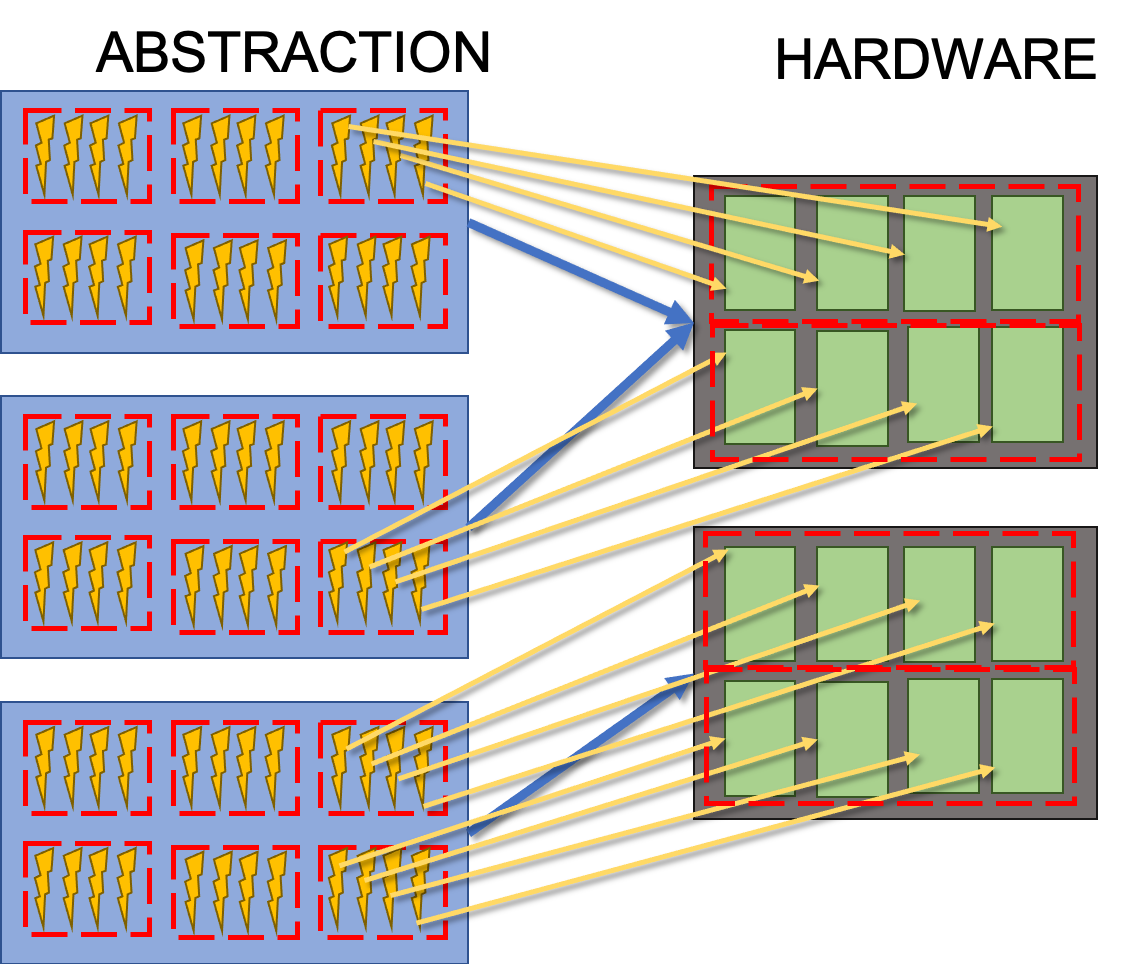
\includegraphics[width=\textwidth]{img/03/gpu-hard-abs.png}
            \end{figure}
        \end{columns}
    \end{frame}

    \begin{frame}{What is shared memory?}
        \begin{itemize}
            \item A variable located in \textbf{shared memory} is ``block private.''
            \begin{itemize}
                \item Each block has a different copy.
                \item All threads in the block have access to that copy.
            \end{itemize}
            \item Within each block, threads may need to be explicitly synchronized to avoid race conditions on shared memory writes.
            \item Shared memory physically resides on higher-bandwidth memory and can be managed by the user.
        \end{itemize}
    \end{frame}
    
    \section{Example: Dot Product}
    
    \subsection{Algorithm}

    \begin{frame}{Extended Example: Dot Product}
        \begin{itemize}
            \item A dot product is one example of a reduction:
            \begin{equation*}
                \vec{a} \cdot \vec{b} = \sum_i = a_i b_i
            \end{equation*}
            \item We will shared-memory buffers to optimize this reduction.
            \item Optimizations are applicable to other reductions, too.
        \end{itemize}
    \end{frame}

    \begin{frame}{Dot Product Algorithm: Step 1}
        \begin{itemize}
            \item The grid dimension is 3 (i.e., 3 total blocks).
            \item The block dimension is 4 (i.e., 4 threads/block).
            \item The operands $a$ and $b$ are in global memory.  They are accessible by all the blocks, but we will organize the accesses so that portions of the arrays are accessed by specific blocks (blue, green and red)
            \item Each block has a shared memory buffer that is private to the block.  Each will store a portion of the results $a_i \times b_i$ before we reduce them.
        \end{itemize}
        \begin{figure}
            \centering
            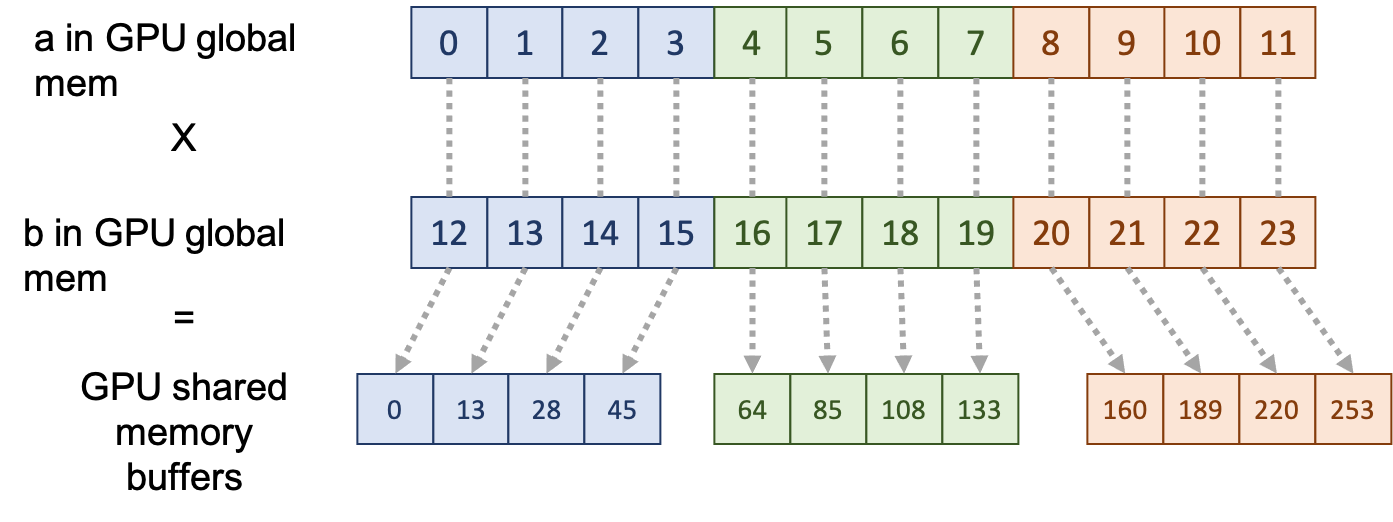
\includegraphics[width=0.8\textwidth]{img/04/dot-01.png}
        \end{figure}
    \end{frame}

    \begin{frame}{Dot Product Algorithm: Step 2}
        \begin{itemize}
            \item Each block performs a reduction (sum) on its shared memory buffer.
            \item Each block puts its partial sum in global memory.
        \end{itemize}
        \begin{figure}
            \centering
            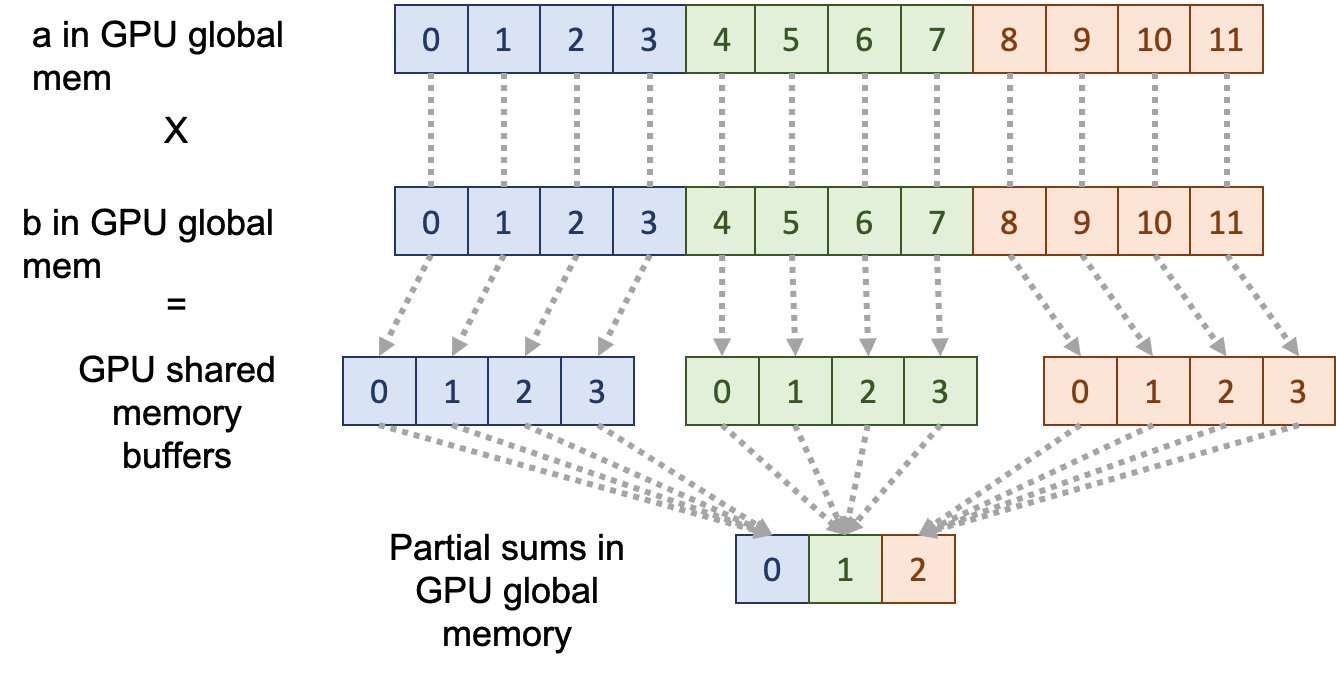
\includegraphics[width=0.8\textwidth]{img/04/dot-02.png}
        \end{figure}
    \end{frame}

    \begin{frame}{Dot Product Algorithm: Step 3}
        \begin{itemize}
            \item The partial sums are sent to the host.
            \item Then the host does the final reduction.
            \item For a very large number of blocks, the reduction is more efficient on the host than the device.
        \end{itemize}
        \begin{figure}
            \centering
            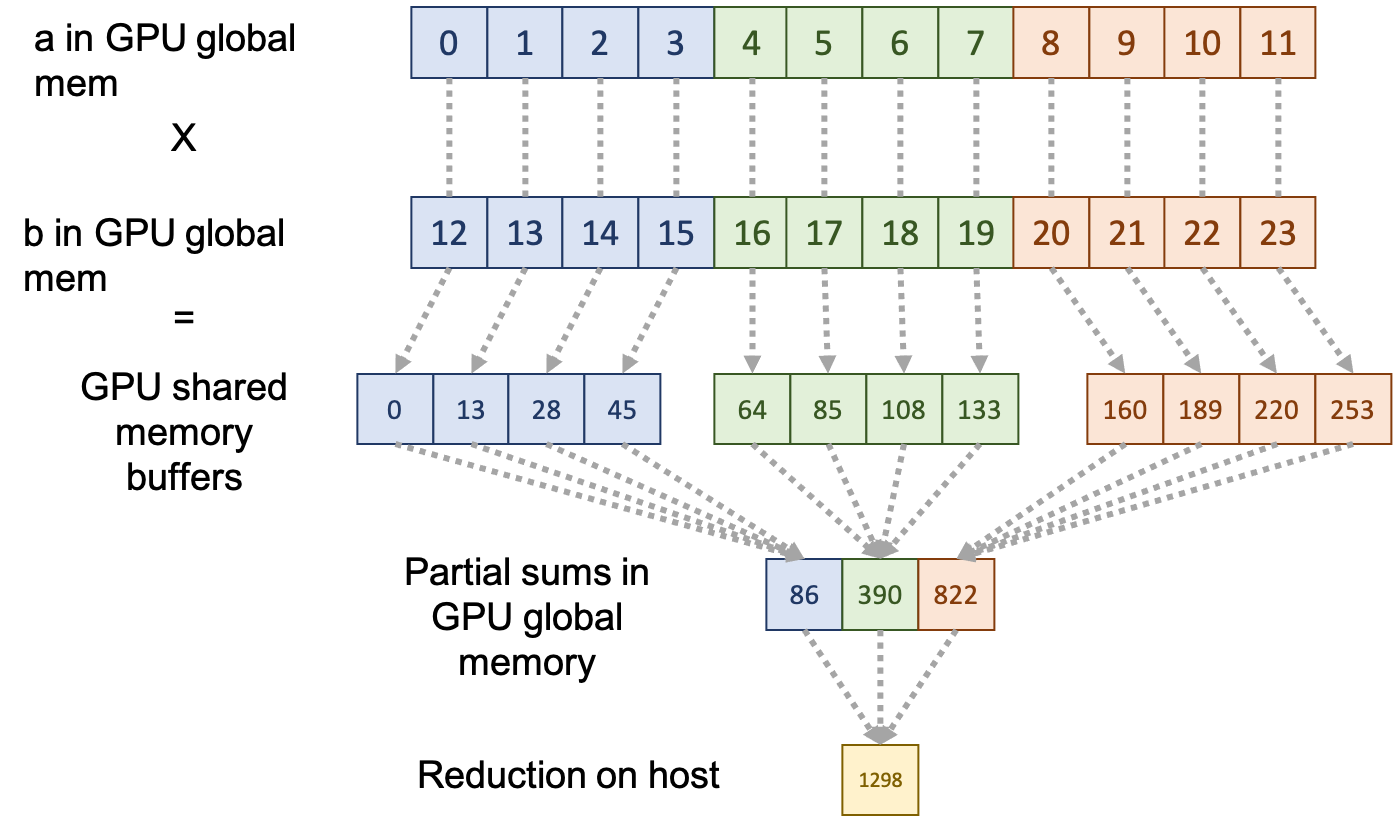
\includegraphics[width=0.8\textwidth]{img/04/dot-03.png}
        \end{figure}
    \end{frame}
    
    \subsection{Implementation}

    \begin{frame}{Completed Example}
        See course repo:  \url{https://github.com/mpcs-hpc/mpcs-hpc-winter-2021/blob/main/week04/dot_static_shared.cu}
    \end{frame}

    \begin{frame}{Part 1. Allocating Memory}
            \begin{itemize}
            {\footnotesize
                \item \texttt{block\_dim} (the number of threads/block) is a compile-time constant
                \item \texttt{n} is the length of the operands \texttt{a} and \texttt{b}
                \item \texttt{grid\_dim} (the number of blocks) is \texttt{ceil(n / block\_dim)}
                \item \texttt{partial\_c} and \texttt{d\_partial\_c} will contain the partial sums from all blocks.
            }
            \end{itemize}
            \begin{block}{}
                \inputminted[fontsize=\footnotesize]{cuda}{src/dot_snippet_01.cu}
            \end{block}
    \end{frame}

    \begin{frame}{Part 2. Each thread computes and its partial result}
        \begin{itemize}
        {\footnotesize
        \item Each block gets a shared memory \texttt{cache} of size \texttt{block\_dim}
        \item Each thread independently accumulates \texttt{cache[threadIdx.x] += a[i] * b[i]} for its subsets of \texttt{a} and \texttt{b}
        \item After this, we want all threads to see the final result their block's \texttt{cache}.  Hence, we sync all the threads in the block with \texttt{\_\_syncthreads()}
        }
        \end{itemize}
        \begin{block}{}
            \inputminted[fontsize=\footnotesize]{cuda}{src/dot_snippet_02.cu}
        \end{block}
    \end{frame}

    \begin{frame}{Part 3.  Parallel reduction in each block}
        \begin{enumerate}
        {\footnotesize
            \item Start with \texttt{block\_dim} values in cache.
            \item \texttt{block\_dim / 2} threads participate in this step.
            \item Each thread will accumulate two values in parallel.
            \item When all threads are done, there are \texttt{block\_dim / 2} results in cache
            \item Continue bisecting until we have 1 result in each block.
        }
        \end{enumerate}
        \begin{figure}
            \centering
            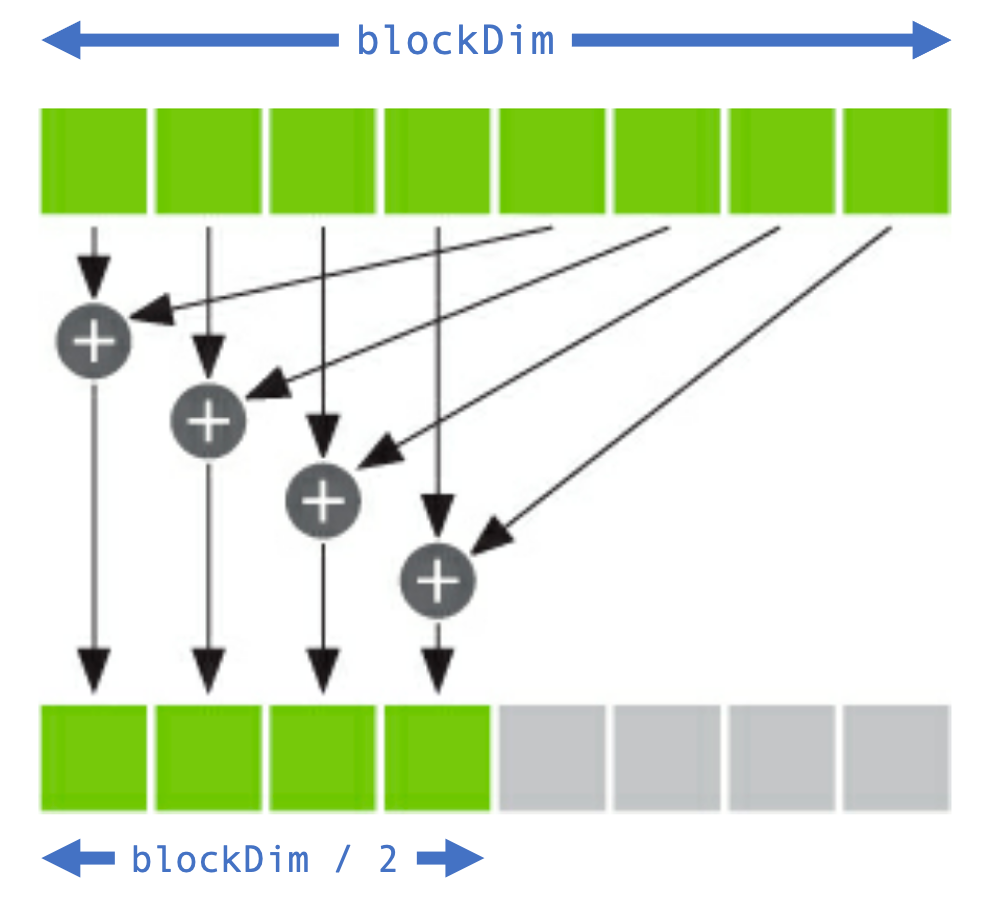
\includegraphics[width=0.5\textwidth]{img/04/parallel-reduc-annotated.png}
        \end{figure}
    \end{frame}

    \begin{frame}{Part 3. Parallel reduction in each block}
        \begin{itemize}
        {\footnotesize
        \item First, do parallel reduction. Note \texttt{\_\_syncthreads()} in each step.
        \item Then each block stores its result in global memory.  This will be sent back to host.
        }
        \end{itemize}
        \begin{block}{}
            \inputminted[fontsize=\footnotesize]{cuda}{src/dot_snippet_03.cu}
        \end{block}
    \end{frame}

    \begin{frame}{Part 4. Parallel reduction on host}
        \begin{itemize}
        {\footnotesize
        \item Recall that \texttt{partial\_c} are the results from each block.
        \item After copying \texttt{partial\_c} to the host, the host does one final reduction.
        \item We could've done the final reduction on device using atomic operations.
              However, for large block counts, atomic operations on device are very inefficient.
              Hence, the host will actually be more efficient for this part.
        }
        \end{itemize}
        \begin{block}{}
            \inputminted[fontsize=\footnotesize]{cuda}{src/dot_snippet_04.cu}
        \end{block}
    \end{frame}


    \begin{frame}{Static Shared Memory}
        Review from dot product in Lecture 4B:
        \begin{itemize}
            \item In global scope:  Declare block dimension
            \begin{block}{}
                \inputminted{cuda}{src/static_01.cu}
            \end{block}
            \item In kernel def:  Declare static array for shared mem
            \begin{block}{}
                \inputminted{cuda}{src/static_02.cu}
            \end{block}
            \item At kernel call:  Determine grid dimension
            \begin{block}{}
                \inputminted{cuda}{src/static_03.cu}
            \end{block}
        \end{itemize}
        See full source in repo, \texttt{src/lecture\_05/dot\_gpu.cu}
    \end{frame}

    \begin{frame}{Dynamic Shared Memory}
        \begin{itemize}
            \item In the kernel definition, a special declaration allows you to use arbitrarily-sized shared memory arrays (note empty brackets)
            \begin{block}{}
                \inputminted{cuda}{src/shared_01.cu}
            \end{block}
            \item In kernel launch, a third config parameter specifies the size of the shared memory per block
            \begin{block}{}
                \inputminted{cuda}{src/shared_02.cu}
            \end{block}
            \item See \url{https://devblogs.nvidia.com/using-shared-memory-cuda-cc/}
        \end{itemize}
    \end{frame}

    \begin{frame}{(Ungraded) Exercise: Implementing Dynamic Shared Memory in Dot Product}
        Start with source in repo, \texttt{src/lecture\_05/dot\_gpu.cu}, and add
        the following features:
        \begin{enumerate}
            \item Add these command line args (don't have to use \texttt{get\_input})
            \begin{itemize}
                \item Size of \texttt{a} and \texttt{b}
                \item Grid dimension
                \item Block dimension
            \end{itemize}
            \item Use command-line args to set size of shared-memory cache
        \end{enumerate}
        Solution in course repo: \url{https://github.com/mpcs-hpc/mpcs-hpc-winter-2021/blob/main/week04/solutions/dot_dynamic_shared.cu}
    \end{frame}

    \section{References}

    \begin{frame}{References}
        \begin{itemize}
            \item Sanders and Kandrot.  \textit{CUDA by Example: An Introduction to General-Purpose GPU Programming}.
            Chapter 5, ``Thread Cooperation''
            \item NVIDIA Developer Blog.  ``Using Shared Memory in CUDA C/C++''  \url{https://developer.nvidia.com/blog/using-shared-memory-cuda-cc/}
            \item CUDA Toolkit Documentation.  ``9.2.3: Shared Memory''  \url{https://docs.nvidia.com/cuda/cuda-c-best-practices-guide/index.html\#shared-memory}
        \end{itemize}
    \end{frame}

\end{document}
